\documentclass{article}
\usepackage{tikz}

\begin{document}

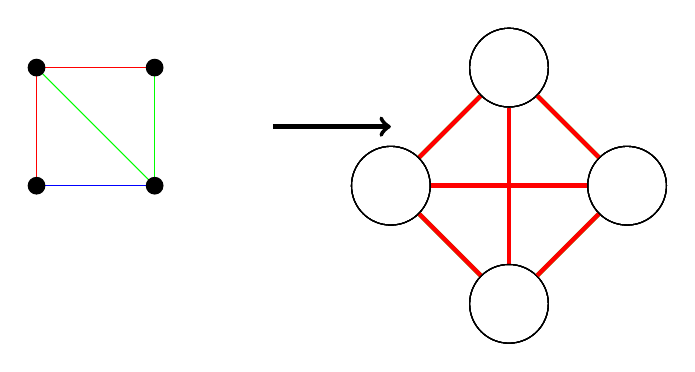
\begin{tikzpicture}[scale=1.5]

% Draw the initial K_4 graph
\draw[blue] (0,0) -- (1,0);
\draw[red] (0,0) -- (0,1);
\draw[green] (0,1) -- (1,0);
\draw[blue] (1,0) -- (1,1);
\draw[red] (0,1) -- (1,1);
\draw[green] (1,0) -- (1,1);

\filldraw[black] (0,0) circle (2pt);
\filldraw[black] (1,0) circle (2pt);
\filldraw[black] (0,1) circle (2pt);
\filldraw[black] (1,1) circle (2pt);

% Draw the thick edges
\draw[ultra thick, blue] (0.5,0.5) -- (0.5,0.5);
\draw[ultra thick, red] (0.5,0.5) -- (0.5,0.5);
\draw[ultra thick, green] (0.5,0.5) -- (0.5,0.5);

% Draw the arrow
\draw[->, ultra thick] (2,0.5) -- (3,0.5);

% Draw the iterated blowup
\begin{scope}[xshift=4cm]
    \foreach \i in {0,...,3} {
        \node[circle, draw, minimum size=1cm] (A\i) at ({90+90*\i}:1) {};
        \foreach \j in {0,...,3} {
            \node[circle, draw, minimum size=1cm] (B\j) at ({90+90*\j}:1) {};
            \ifnum\i=\j
                \draw[ultra thick, blue] (A\i) -- (B\j);
            \else
                \ifnum\i<\j
                    \draw[ultra thick, green] (A\i) -- (B\j);
                \else
                    \draw[ultra thick, red] (A\i) -- (B\j);
                \fi
            \fi
        }
    }
\end{scope}

\end{tikzpicture}

\caption{Iterated blowup of a \(K_4\). The ``thick'' edges indicate that all possible edges between the sets of vertices are given the specified color.}

\end{document}